\documentclass[11pt,a4paper]{article}
\usepackage[english]{babel}
\usepackage[a4paper,margin=1in]{geometry}
\usepackage[T1]{fontenc}
\usepackage{lmodern}
\usepackage{microtype}
\usepackage{csquotes}
\usepackage{amsmath,amssymb,booktabs,tabularx,array,graphicx}
\usepackage{enumitem}
\usepackage[most]{tcolorbox}
\usepackage{multicol}
\usepackage{wrapfig}
\usepackage[hidelinks]{hyperref}
\usepackage[compact]{titlesec}
\usepackage[font=small,skip=4pt]{caption}
\usepackage{listings}
\lstset{basicstyle=\ttfamily\scriptsize,breaklines=true,frame=single,columns=fullflexible}
\titlespacing*{\section}{0pt}{8pt}{4pt}
\titlespacing*{\subsection}{0pt}{6pt}{2pt}
\setlength{\textfloatsep}{8pt plus 2pt minus 2pt}
\setlength{\floatsep}{8pt plus 2pt minus 2pt}
\setlength{\intextsep}{8pt plus 2pt minus 2pt}
\setlength{\parskip}{1pt}
\graphicspath{{images/}{report/figures/}}

% ---------------------------------------------------------------------------
%  Boxes
% ---------------------------------------------------------------------------
\newtcolorbox{kaobox}[1][]{
  colback=gray!5,
  colframe=gray!55,
  boxrule=0.5pt,
  arc=2pt,
  left=6pt, right=6pt, top=6pt, bottom=6pt,
  #1
}

% ---------------------------------------------------------------------------
%  Shorthand
% ---------------------------------------------------------------------------
\newcommand{\sir}{\mathrm{SIR}}
\newcommand{\gnode}{\mathrm{GN\text{-}ODE}}
\newcommand{\dmp}{\mathrm{DMP}}
\newcommand{\gcn}{\mathrm{GCN}}

\begin{document}
\hypersetup{pageanchor=false}

% ===========================================================================
%  TITLE PAGE
% ===========================================================================
\begin{titlepage}
\centering
\vspace*{0.8cm}

\vfill

\rule{\linewidth}{0.5pt}\\[0.7cm]
{\Huge\bfseries Understanding Neural Ordinary Differential Equations\par}
\vspace{0.5cm}
{\LARGE From Simple  Models to Network Epidemics\par}
\vspace{0.7cm}
\rule{\linewidth}{0.5pt}

\vfill

{\large\bfseries Bachelor Seminar}\\[1.6cm]

\begin{tabular}{rl}
\textbf{Presented by} & Veronika Rybak \\[4pt]
\textbf{Supervisor}   & Prof.\ Dr.\ Nadja Ray \\
\end{tabular}

\vfill
{\footnotesize\today}
\end{titlepage}

\hypersetup{pageanchor=true}

% ===========================================================================
%  FRONT MATTER
% ===========================================================================
\pagenumbering{roman}
\tableofcontents
\newpage
\pagenumbering{arabic}

\begin{kaobox}[title=Central question of the seminar]
\emph{How can a neural network learn a differential equation?}
A Neural Ordinary Differential Equation does not learn the solution of a system
directly; it learns the rule by which the system changes, and an ODE solver turns
that rule into trajectories. This report builds up this idea on two small
examples that can be checked completely, exponential decay and the SI epidemic
model, and then follows it to a research model for epidemic spreading on contact
networks.
\end{kaobox}

\section*{Abstract}
\addcontentsline{toc}{section}{Abstract}

This report summarizes a bachelor seminar on Neural Ordinary Differential
Equations (Neural ODEs). The first part introduces the necessary theory of
ordinary differential equations, initial value problems, vector fields, and the
Euler method, and explains the Neural ODE as a learned right-hand side of an
ODE. Each concept is illustrated on the exponential decay equation, including a
one-parameter Neural ODE that learns the decay rate.

The second part uses a sequence of controlled numerical experiments to make
the learning process observable. First, a single unknown decay rate is
estimated from trajectory data. Next, a small neural network learns the
complete scalar decay rule without being given derivative labels. The same
construction is then transferred to the two-dimensional SI epidemic model,
where the learned rule is also tested from a new initial condition. Because
the underlying equations are known in all of these examples, the learned
dynamics can be compared directly with the ground truth.

The final part uses this vocabulary to interpret the Graph Neural ODE
(GN-ODE) model of Kosma et al.\ (2023) for epidemic spreading on contact
networks. The purpose of this progression is to understand the Neural ODE
mechanism first on systems that can be checked completely, before applying
the same ideas to a graph-based model.


\section{ODE Foundations}

\subsection{Ordinary Differential Equations}

An Ordinary Differential Equation (ODE) describes how a quantity changes over
time instead of directly giving its value. A common first-order ODE has the form
\begin{equation}
  \frac{dy(t)}{dt} = f\bigl(y(t),t\bigr),
  \label{eq:ode}
\end{equation}
where $y(t)$ is the state of the system at time $t$, $dy(t)/dt$ is its rate of
change, and $f$ defines how the system evolves. The unknown in an ODE is a
\emph{function} $y(t)$ rather than a single number, which is the main difference
from an algebraic equation. The word \emph{ordinary} means that the equation
contains derivatives with respect to only one independent variable, here time.

The key idea is that an ODE provides a \emph{local rule of motion}. If we know
the current state and the current time, the equation tells us in which direction
and how fast the state is changing at that moment only; it does not tell us the whole
curve. This idea appears in many applications, including population growth,
radioactive decay, and the motion of a pendulum.

\subsection{A simple scalar ODE: exponential decay}

A well-known example is exponential decay, where a quantity decreases at a rate
proportional to its current value:
\begin{equation}
  \frac{dy}{dt} = -\lambda y, \qquad \lambda > 0 .
  \label{eq:decay}
\end{equation}
Here $f(y,t) = -\lambda y$ does not depend on $t$ explicitly. Its analytical
solution, obtained by separating the variables, is
\begin{equation}
  y(t) = y_0\, e^{-\lambda t}.
  \label{eq:decay-sol}
\end{equation}
Since the rate of change is proportional to the current value, larger values
decrease faster than smaller ones. As a result, the curve becomes flatter as it
approaches zero. The parameter $\lambda$ controls how quickly this happens.

Exponential decay is used as a running example throughout the first part of the
report: every concept introduced below (initial value problems, vector fields,
numerical solvers, and finally the Neural ODE itself) is first illustrated on
Equation~\eqref{eq:decay}.

\subsection{Initial value problems}

An ODE alone does not determine a single trajectory. For the decay equation, every
function $y(t) = C e^{-\lambda t}$ solves \eqref{eq:decay}, for any constant $C$.
To select one solution, an initial condition is needed. Together,
\begin{equation}
  \frac{dy}{dt} = f(y,t), \qquad y(t_0) = y_0
  \label{eq:ivp}
\end{equation}
form an \emph{initial value problem} (IVP). The ODE defines \emph{how} the system
changes, while the initial condition determines \emph{where} it begins. In the
decay example, $y(0) = y_0$ fixes $C = y_0$ and yields \eqref{eq:decay-sol}.

If $f$ is continuous in $t$ and locally Lipschitz continuous in $y$, then
for every initial condition there exists a unique solution, at least locally
around the initial time (Picard--Lindel\"of theorem). Thus, on an interval
where the solution exists, a given initial state determines one unique
trajectory. This is important for Neural ODEs, where the input is used as the
initial state of an initial value problem.

\subsection{From local derivatives to trajectories}

An ODE tells us how the system changes at its current state. For a scalar
equation such as exponential decay,
\[
    \frac{dy}{dt}=-\lambda y,
\]
the value $-\lambda y$ gives the slope of the trajectory at the current value
of $y$. When $y$ is large, the slope is more negative; as $y$ approaches zero,
the slope becomes smaller. This explains why the decay curve becomes flatter
over time.

For a system with several variables, the state is a vector
$y(t)\in\mathbb{R}^d$, and the function $f$ returns a vector of derivatives.
These derivative vectors describe the direction in which the state moves.
Taken together, they form a \emph{vector field}.

The idea of a vector field is important for Neural ODEs because the neural
network will later play exactly this role: it will learn a function
$f_\theta$ that takes the current state and returns its derivative. A concrete
two-dimensional derivative function will be used later for the SI epidemic model.

Knowing the derivative at one point is not yet the same as knowing the whole
trajectory. To obtain the trajectory, an ODE solver repeatedly evaluates the
derivative and moves the state forward in time. The simplest example is the
forward Euler method,
\begin{equation}
    y_{n+1}=y_n+h\,f(y_n,t_n),
    \label{eq:euler}
\end{equation}
where $h$ is the step size.

For exponential decay this becomes
\begin{equation}
    y_{n+1}=y_n-h\lambda y_n.
\end{equation}
Starting from $y_0$, Euler's method repeatedly uses the current slope to
approximate the next value. Smaller step sizes usually follow the exact decay
curve more closely, as shown in Figure~\ref{fig:euler}. In this experiment,
the maximum absolute error is $0.089$ for $h=0.5$ and $0.0075$ for $h=0.05$.

The source code used for all numerical experiments and generated figures is
provided in the accompanying GitHub repository and listed in
Appendix~\ref{app:code}.

\begin{figure}[h]
    \centering
    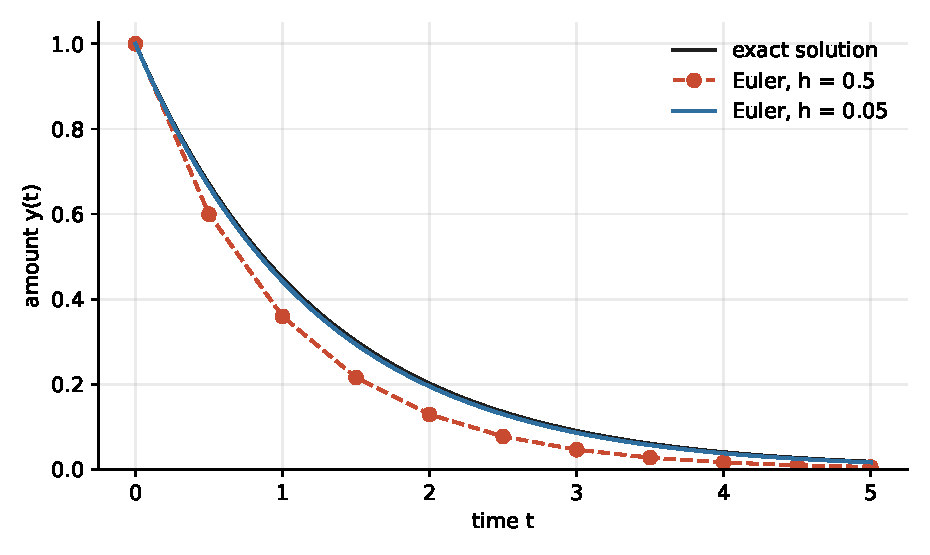
\includegraphics[width=0.78\textwidth]{01_euler_decay.pdf}
    \caption{Euler's method applied to $y'=-0.8y$, $y(0)=1$. The approximation
    with $h=0.05$ follows the exact solution more closely than the approximation
    with $h=0.5$.}
    \label{fig:euler}
\end{figure}

This separation between the two tasks will be important later: the function
$f$ provides the local derivative, while the numerical solver uses these
derivatives to construct the trajectory.

% =====================================================================
\section{From Numerical Solvers to Neural ODEs}

\subsection{Residual networks as motivation}

The historical motivation for Neural ODEs comes from residual networks. A
residual block updates a hidden state according to
\begin{equation}
    h_{k+1}=h_k+F_k(h_k;\theta_k),
\end{equation}
which has the same algebraic form as one Euler step,
\[
    y_{n+1}=y_n+h f(y_n,t_n):
\]
the new state is the current state plus a change computed from that state.

This observation suggests interpreting the layer index $k$ as a discrete time
variable. A residual network can then be viewed as a discrete dynamical system.
Neural ODEs take the corresponding continuous limit: instead of specifying one
update for each discrete layer, a single function $f_\theta$ specifies the
instantaneous rate of change continuously in time. This connection explains the motivation behind Neural ODEs. From this point
on, however, we will focus directly on the ODE viewpoint: the neural network
defines the derivative, and the numerical solver constructs the trajectory.

\subsection{The Neural ODE: core formulation}

A Neural ODE replaces a sequence of discrete updates by a continuous
dynamical system. Instead of moving through states
\[
    h_0 \to h_1 \to \cdots \to h_L,
\]
the state evolves continuously according to
\begin{equation}
    \frac{dh(t)}{dt}
    =
    f_\theta\bigl(h(t),t\bigr),
    \label{eq:node}
\end{equation}
where $f_\theta$ is a neural network with trainable parameters $\theta$.

The role of $f_\theta$ is the same as the function $f$ in an ordinary
differential equation: given the current state, it returns the instantaneous
rate of change. Starting from an initial state $h(0)$, an ODE solver repeatedly
evaluates $f_\theta$ and uses these derivatives to construct the trajectory
$h(t)$.

Formally, the state at a later time $T$ satisfies
\begin{equation}
    h(T)
    =
    h(0)
    +
    \int_0^T
    f_\theta\bigl(h(t),t\bigr)\,dt .
    \label{eq:odesolve}
\end{equation}

The important difference from an ordinary neural network is therefore that
$f_\theta$ does not directly compute the final output. It defines how the
state changes locally, while the ODE solver combines these local changes to
produce the trajectory.

\paragraph{A simple trainable example: exponential decay.}

The exponential-decay example can be used to show the learning idea in the
simplest possible setting. Suppose the true system is
\[
    \frac{dy}{dt}=-\lambda y,
\]
but the decay rate $\lambda$ is unknown. We replace it by a trainable
parameter $\theta$ and use
\begin{equation}
    f_\theta(y)=-\theta y.
    \label{eq:toy-field}
\end{equation}

The resulting model is
\[
    \frac{dy}{dt}=-\theta y,
    \qquad
    y(0)=y_0.
\]
For a given value of $\theta$, the ODE solver produces a trajectory. This
trajectory can be compared with observed data, and $\theta$ can then be
adjusted to reduce the difference. If the data were generated using the true
decay rate $\lambda$, training should recover a value of $\theta$ close to
$\lambda$.

This example does not yet learn an unknown functional form: the structure
$-\theta y$ is already built into the model, and only one parameter is
learned. Its purpose is to make the Neural ODE training idea transparent
before moving to a neural network that learns the derivative function itself.

\subsection{What the network learns}

A Neural ODE learns the function $f_\theta$ that describes how the current
state changes. The ODE solver then uses this function to construct the
trajectory.

In the exponential-decay example,
\[
    f_\theta(y)=-\theta y,
\]
so training changes the parameter $\theta$. Once $\theta$ has been learned,
the same differential equation can be solved from different initial values
$y_0$. The initial value determines where the trajectory starts, while
$f_\theta$ determines how it evolves.

For this simple example, the functional form $-\theta y$ is already known and
only the decay rate is learned. Later, in the SI example, $f_\theta$ will also
be represented by a neural network, so that more of the derivative function
can be learned from data.

\subsection{Training a Neural ODE}

Training changes the parameters $\theta$ of the derivative function
$f_\theta$. The basic procedure is:

\begin{enumerate}
    \item[(1)] \textbf{Forward solve:}
    starting from the initial state, the ODE solver uses the current
    $f_\theta$ to produce a predicted trajectory.

    \item[(2)] \textbf{Loss:}
    the predicted states are compared with the observed data. For example,
    for observations $y^*(t_k)$ we can use
    \[
        L(\theta)
        =
        \sum_k
        \left(
            y_\theta(t_k)-y^*(t_k)
        \right)^2 .
    \]

    \item[(3)] \textbf{Gradient computation:}
    the loss is differentiated with respect to the parameters $\theta$.

    \item[(4)] \textbf{Parameter update:}
    the parameters are changed in a direction that reduces the loss,
    \[
        \theta
        \leftarrow
        \theta-\eta\frac{\partial L}{\partial\theta},
    \]
    where $\eta$ is the learning rate.
\end{enumerate}

The important point is that training does not directly modify the trajectory.
It modifies $f_\theta$. When the ODE is solved again with the updated
$f_\theta$, a different trajectory is produced.

\paragraph{Experiment: recovering the decay rate.}

Noiseless observations were generated from Equation~\eqref{eq:decay-sol} with
$\lambda=0.8$, $y_0=1$, at times $0,0.5,\ldots,5$. The trainable model
$f_\theta(y)=-\theta y$ started from $\theta=0.3$. It was trained for
$2{,}000$ updates using Adam with learning rate $0.001$, while Euler's method
with $h=0.01$ was used inside the loss.

After training, the learned value was $\theta=0.786$ and the mean squared
trajectory error was $9.9\cdot10^{-6}$. The result is close to the true rate,
but it is important that the functional form $-\theta y$ was supplied in
advance. Only one coefficient was learned.

\begin{figure}[h]
    \centering
    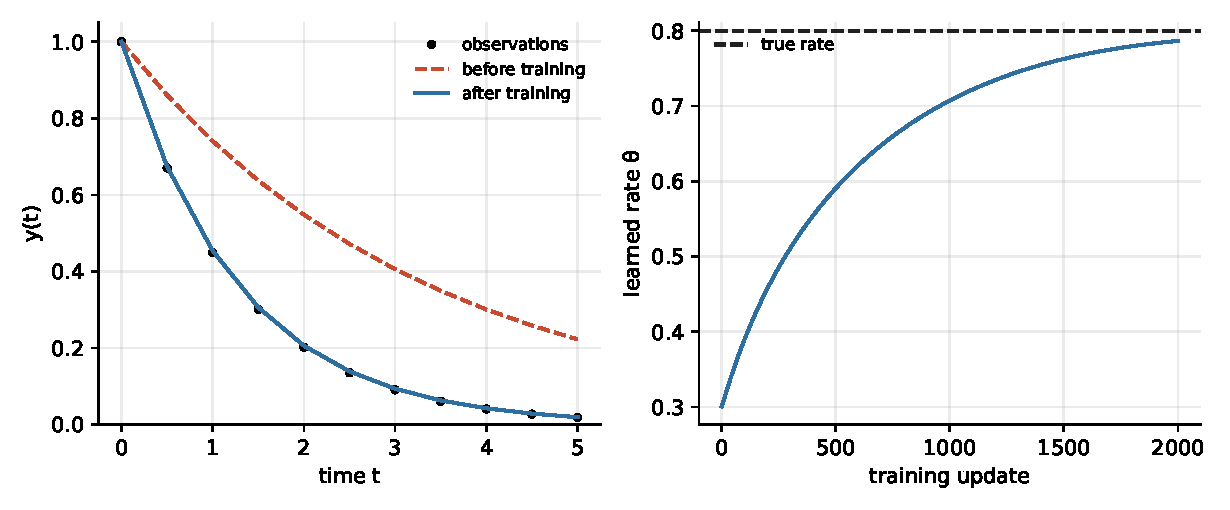
\includegraphics[width=0.95\textwidth]{02_decay_parameter_learning.pdf}
    \caption{Learning the parameter of $dy/dt=-\theta y$. Left: observations
    and trajectories before and after training. Right: the learned parameter
    approaches the true decay rate $\lambda=0.8$.}
    \label{fig:toy}
\end{figure}

\subsection{Learning the decay rule with a neural network}
\label{sec:neural-decay}

The previous experiment already knew the form of the equation. To learn more
than one parameter, we now replace $-\theta y$ by a small neural network,
\[
    \frac{dy}{dt}=f_\theta(y).
\]
The network has one input, one hidden layer with 16 tanh units, and one linear
output. Its input is the current value $y$, and its output is the proposed
derivative. Training uses the same decay observations and the same Euler solver
as the previous experiment. The true derivative values $-0.8y$ are not used as
training labels.

Figure~\ref{fig:neural-decay} compares the learned result with the known
system. The final trajectory loss is $1.0\cdot10^{-5}$. On the range of $y$
visited by the trajectory, the mean squared difference between the learned and
true derivatives is $2.2\cdot10^{-4}$. Thus the experiment shows directly how
trajectory observations can train a function that represents a derivative.
The comparison only supports the learned rule on the observed range; it does
not test states far outside that range.

\begin{figure}[h]
    \centering
    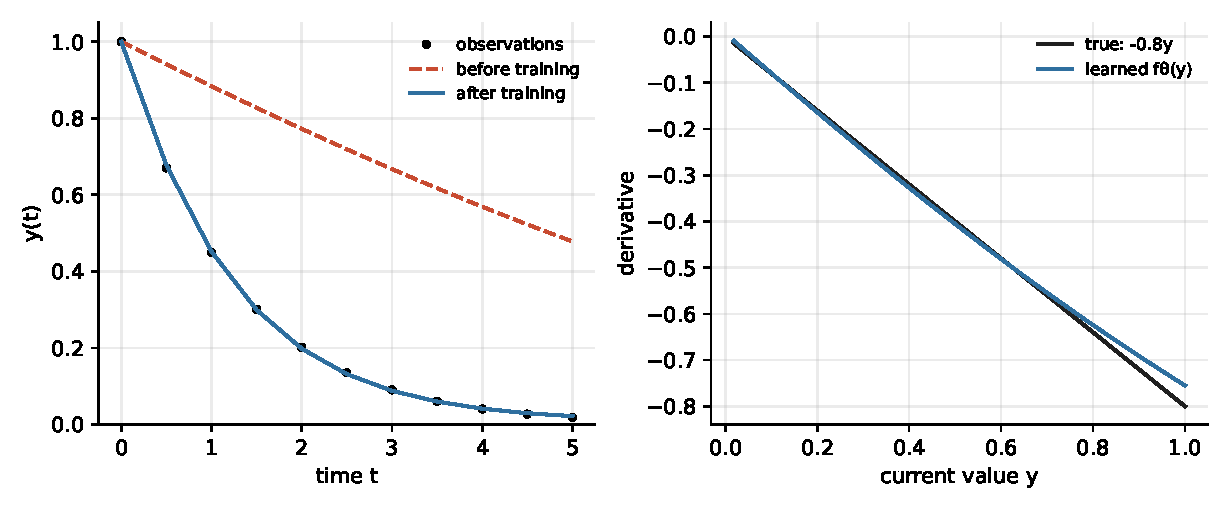
\includegraphics[width=0.95\textwidth]{03_decay_neural_rule.pdf}
    \caption{Learning the complete decay rule. Left: the trajectory before and
    after training. Right: the learned derivative $f_\theta(y)$ compared with
    the true derivative $-0.8y$ on the observed range.}
    \label{fig:neural-decay}
\end{figure}


\section{From Exponential Decay to the SI Model}
\label{sec:si}
\subsection{The SI model as a two-dimensional ODE}

So far, the state of the system was a single number $y(t)$. To move toward
epidemic dynamics, we now consider a system with two state variables.

In the SI model, individuals are either susceptible ($S$) or infected ($I$),
and infected individuals do not recover. We work with population fractions, so
\begin{equation}
    S(t)+I(t)=1.
    \label{eq:si-conservation}
\end{equation}

The dynamics are
\begin{equation}
    \frac{dS}{dt}=-\beta SI,
    \qquad
    \frac{dI}{dt}=\beta SI,
    \label{eq:si}
\end{equation}
where $\beta>0$ controls the infection rate.

The same quantity $\beta SI$ leaves the susceptible group and enters the
infected group. Therefore
\begin{equation}
    \frac{d}{dt}(S+I)=0,
\end{equation}
which explains the conservation law $S+I=1$.

The important step for this report is that the state is now a vector,
\[
    \mathbf{x}
    =
    \begin{pmatrix}
        S\\I
    \end{pmatrix}.
\]
The two equations can therefore be written as one vector-valued ODE,
\begin{equation}
    \frac{d\mathbf{x}}{dt}
    =
    \begin{pmatrix}
        -\beta SI\\
         \beta SI
    \end{pmatrix}
    =
    f(\mathbf{x}).
    \label{eq:si-vector}
\end{equation}

Compared with exponential decay, nothing fundamental has changed: $f$ still
describes the local rate of change, but it now returns two derivatives instead
of one.

For example, for $\beta=1$ and $(S,I)=(0.8,0.2)$,
\[
    f(0.8,0.2)=(-0.16,\,0.16).
\]
At this state, the susceptible fraction decreases at rate $0.16$ while the
infected fraction increases at the same rate. In two dimensions, the
collection of such derivative vectors is called a vector field.

Because $S=1-I$, the SI system can also be reduced to
\[
    \frac{dI}{dt}=\beta I(1-I),
\]
with analytical solution
\begin{equation}
    I(t)=
    \frac{1}{1+\frac{1-I_0}{I_0}e^{-\beta t}},
    \qquad
    S(t)=1-I(t).
    \label{eq:si-solution}
\end{equation}
This known solution will be used as the reference trajectory for the Neural
ODE experiment. The purpose of the SI model here is therefore not to study
epidemic modelling in detail, but to test the same Neural ODE idea on a
nonlinear state with two components.

\section{Turning the SI Model into a Neural ODE}
\label{sec:si-node}

The neural-decay experiment used a neural network
\[
    f_\theta:\mathbb{R}\rightarrow\mathbb{R}
\]
to learn a scalar derivative. The SI model uses exactly the same construction,
but the state now has two components.

With
\[
    \mathbf{x}=(S,I)^\top,
\]
we replace the known SI right-hand side by
\begin{equation}
    \dot{\mathbf{x}}
    =
    f_\theta(\mathbf{x}),
    \qquad
    f_\theta:\mathbb{R}^2\rightarrow\mathbb{R}^2.
    \label{eq:si-node}
\end{equation}

At each evaluation, the neural network receives the current values $(S,I)$
and returns two numbers,
\[
    f_\theta(S,I)
    =
    \begin{pmatrix}
        \dot S\\
        \dot I
    \end{pmatrix}.
\]
The ODE solver then repeatedly evaluates these derivatives to construct
$S(t)$ and $I(t)$. Thus the computation is
\[
    (S,I)
    \xrightarrow{\,f_\theta\,}
    (\dot S,\dot I)
    \xrightarrow{\text{ODE solver}}
    (S(t),I(t)).
\]

During training, trajectory observations are used to define the loss; the
network is not given the true derivative values as training labels. This is
the direct two-dimensional analogue of the neural-decay experiment in
Section~\ref{sec:neural-decay}.

The next section tests whether this small neural network can learn the SI
dynamics from generated trajectories and whether the same learned rule can be
integrated from a different initial condition.

\section{Experiment: Learning the SI Rule}
\label{sec:si-experiments}

The reference observations are generated analytically from
Equation~\eqref{eq:si-solution} with $\beta=1$ at the integer times on
$t\in[0,15]$. The learned model is intentionally simple: a multilayer
perceptron with inputs $(S,I)$, one hidden layer of 16 tanh units, and outputs
$(\dot S,\dot I)$. It is trained from complete state trajectories rather than
from derivative labels.

\paragraph{Learning the rule.}

The training set contains two trajectories, starting from $I_0=0.01$ and
$I_0=0.10$, with $S_0=1-I_0$. The loss is the mean squared error between the
predicted and reference values of both $S$ and $I$. The solver uses Euler steps
with $h=0.2$, and the network is trained for 500 Adam updates with learning
rate $0.001$.

The right panel of Figure~\ref{fig:si-neural-experiment} compares the learned
and true derivatives along the physically valid line $S=1-I$. The mean squared
derivative error on this line is $0.0106$. The network captures the general
shape of the infection process but does not reproduce the analytical rule
perfectly.

\paragraph{Testing a new initial condition.}
\label{sec:si-new-ic}

After training, the same $f_\theta$ is solved from $I_0=0.05$, without changing
the network parameters. This initial condition was not in the training set but
lies between the two training conditions. The left panel of
Figure~\ref{fig:si-neural-experiment} compares the resulting trajectory with
the analytical solution. Its root mean squared error over $S$ and $I$ is
$0.114$. The prediction follows the overall epidemic trend, although a visible
difference remains.

This result illustrates the role of an initial value problem. A new starting
point does not require a new model: the solver follows the same learned rule
from a different state. At the same time, the result should be interpreted
carefully. All training and test states lie on $S+I=1$, and the test condition
lies inside the range of the training conditions. The experiment therefore
tests interpolation in a familiar region, not arbitrary extrapolation.

\begin{figure}[h]
  \centering
  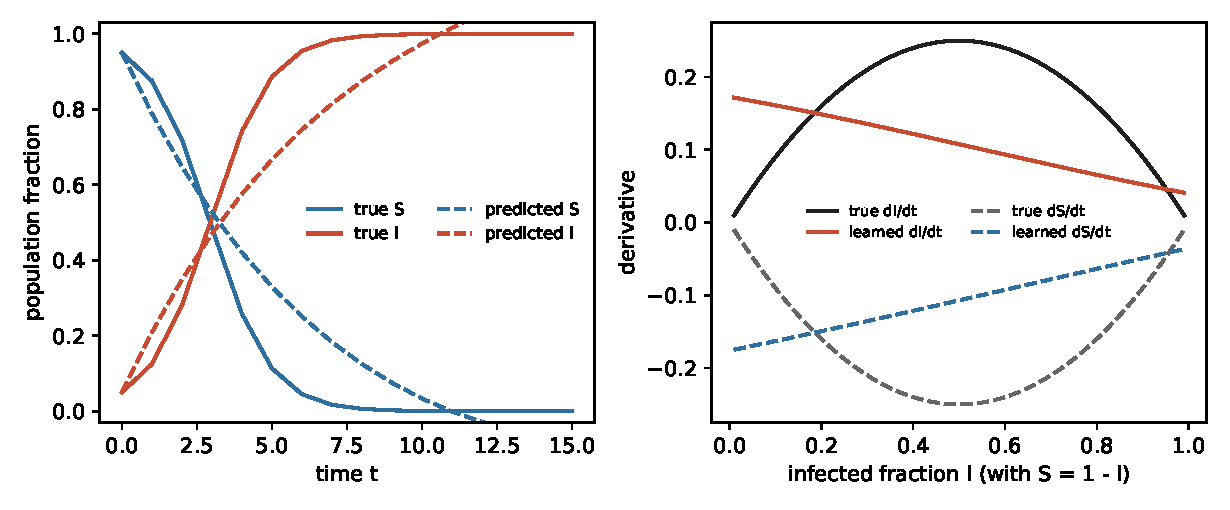
\includegraphics[width=0.95\textwidth]{04_si_neural_rule_and_new_initial_condition.pdf}
  \caption{The learned SI model. Left: analytical and predicted trajectories
  from the unseen initial condition $I_0=0.05$. Right: learned and true
  derivatives along the line $S=1-I$.}
  \label{fig:si-neural-experiment}
\end{figure}

% ===========================================================================
% ===========================================================================
\section{From the SI Model to Epidemic Spreading on Networks}
\label{sec:networks}
% ===========================================================================

The preceding experiments established the mechanism needed for the network
application: a state is passed to a learned derivative function, and an ODE
solver integrates that rule over time. Moving to epidemic spreading on a
network changes the size and structure of the state, but not this basic
principle.

The SI example was deliberately simple: the complete state consisted of only
two numbers, $S(t)$ and $I(t)$, and every individual was treated as part of one
well-mixed population. The application studied by Kosma et al.\ (2023) retains
the same basic idea---describe local rates of change by an ODE---but enlarges
the state in two steps. First, recovery is added. Second, instead of describing
only population fractions, the epidemic state is represented separately for
the nodes of a contact network.


\subsection{Adding recovery: from SI to SIR}

The SI model assumes that an infected individual remains infected forever. The
SIR model adds a recovered state $R$. For population fractions,
\[
    S(t)+I(t)+R(t)=1,
\]
and the dynamics are
\begin{align}
    \frac{dS}{dt} &= -\beta SI, \\
    \frac{dI}{dt} &=  \beta SI-\gamma I, \\
    \frac{dR}{dt} &=  \gamma I .
\end{align}
The new parameter $\gamma>0$ is the recovery rate. The infection term is the
same one already studied in the SI model. The only new process is
\[
    I \longrightarrow R,
\]
which removes infected individuals at rate $\gamma I$.

Thus the move from SI to SIR does not introduce a new modelling principle. It
only enlarges the state from
\[
    \mathbf{x}=(S,I)^\top
\]
to
\[
    \mathbf{x}=(S,I,R)^\top
\]
and changes the vector field accordingly.


\subsection{From one population to one state per node}

The well-mixed equations still assume that every susceptible individual can
interact equally with every infected individual. To model a contact structure,
let
\[
    G=(V,E)
\]
be a graph with $n=|V|$ nodes and adjacency matrix
$A\in\mathbb{R}^{n\times n}$. The entry $A_{ij}$ describes whether node $i$
can interact with node $j$.

\begin{figure}[h]
  \centering
  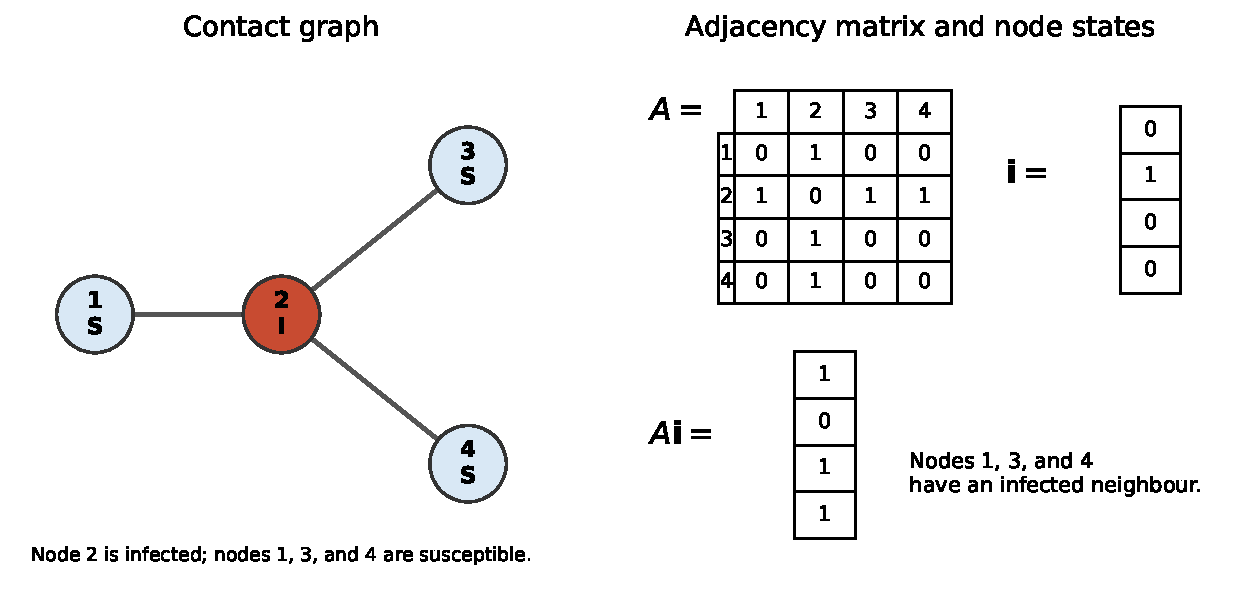
\includegraphics[width=0.90\textwidth]{05_network_example.pdf}
  \caption{A small contact network and its adjacency matrix. With node 2
  infected, the product $A\mathbf{i}$ identifies nodes 1, 3, and 4 as having an
  infected neighbour.}
  \label{fig:network-example}
\end{figure}

For every node $i$, define
\[
    s_i(t),\qquad i_i(t),\qquad r_i(t)
\]
as the probabilities of being susceptible, infectious, and recovered. They
satisfy
\[
    s_i+i_i+r_i=1.
\]
Collecting all nodes gives the vectors
\[
    \mathbf{s},\mathbf{i},\mathbf{r}\in\mathbb{R}^n.
\]

The complete epidemic state can therefore be written as the matrix
\begin{equation}
    X(t)=
    \begin{pmatrix}
        s_1(t) & i_1(t) & r_1(t)\\
        s_2(t) & i_2(t) & r_2(t)\\
        \vdots & \vdots & \vdots\\
        s_n(t) & i_n(t) & r_n(t)
    \end{pmatrix}
    \in\mathbb{R}^{n\times 3}.
    \label{eq:network-state-matrix}
\end{equation}
Each row describes one node and each column one epidemic state.

This is the network analogue of the vector
$(S,I)^\top$ used in Section~\ref{sec:si}. The main difference is dimension:
instead of evolving two population-level variables, the model now evolves
state information for every node.


\subsection{A vector form of the approximate network dynamics}

Under a simple independence approximation, the node-level equations can be
written compactly as
\begin{equation}
    \frac{d}{dt}
    \begin{pmatrix}
        \mathbf{s}\\
        \mathbf{i}\\
        \mathbf{r}
    \end{pmatrix}
    =
    \begin{pmatrix}
        -\beta\,\mathbf{s}\odot(A\mathbf{i})\\[3pt]
         \beta\,\mathbf{s}\odot(A\mathbf{i})-\gamma\mathbf{i}\\[3pt]
         \gamma\mathbf{i}
    \end{pmatrix},
    \label{eq:network-sir-vector}
\end{equation}
where $\odot$ denotes elementwise multiplication.

Equation~\eqref{eq:network-sir-vector} is the direct network counterpart of
Equation~\eqref{eq:si-vector}. The vector $A\mathbf{i}$ has one entry per node.
Its $i$th entry,
\[
    (A\mathbf{i})_i=\sum_j A_{ij}i_j,
\]
summarizes the infectious pressure coming from the neighbours of node $i$.
Multiplying this quantity by $s_i$ gives the rate at which node $i$ loses
susceptibility.

This representation is useful because it shows that moving from the SI model
to a network has not changed the Neural ODE principle. We still have
\[
    \dot{\mathbf{x}}=f(\mathbf{x}),
\]
but $\mathbf{x}$ is now a much larger state and the vector field also depends
on the graph structure $A$.


\subsection{Why an approximation is needed}

The node probabilities are not completely independent. In an exact stochastic
network model, the infection rate of node $i$ depends on joint events such as
the probability that node $i$ is susceptible while a neighbour $j$ is
infected. Tracking all such dependencies becomes expensive because a network
with $n$ SIR nodes has $3^n$ possible global configurations.

A common simplification is therefore to approximate joint probabilities using
lower-dimensional quantities. This makes the system tractable but loses some
correlation information. GN-ODE can be viewed as a model that keeps the
epidemic and graph structure while introducing learned representations to make
the dynamics more flexible.

% ===========================================================================
\section{GN-ODE as an Extension of the Simple Neural ODE}
\label{sec:gnode}
% ===========================================================================

The examples in Sections~\ref{sec:si-node}--\ref{sec:si-experiments} make it
possible to describe the Graph Neural ODE without introducing a completely new
set of concepts.

For the SI experiment, the model had the form
\[
    \dot{\mathbf{x}}=f_\theta(\mathbf{x}),
    \qquad
    \mathbf{x}=(S,I)^\top.
\]
For a network, the same idea becomes schematically
\[
    \dot{X}=f_\theta(X,A),
\]
where $X$ contains the node states and $A$ supplies the information about which
nodes interact.


\subsection{Encode, evolve, decode}

The GN-ODE model of Kosma et al.\ (2023) follows an
\emph{encode--evolve--decode} structure.

First, a trainable encoder transforms the observed node states into hidden
representations. Write the three hidden channels as $S_h$, $I_h$, and $R_h$.
They are not themselves observable probabilities; they are learned quantities
used inside the derivative calculation.

Second, these hidden variables evolve inside an ODE solver. In simplified
notation, their derivative retains the SIR structure,
\begin{align}
    \frac{dS_h}{dt}
        &= -\beta\,(A I_h)\odot S_h,\\
    \frac{dI_h}{dt}
        &=  \beta\,(A I_h)\odot S_h-\gamma I_h,\\
    \frac{dR_h}{dt}
        &=  \gamma I_h.
    \label{eq:gnode-core}
\end{align}
Here the multiplication $A I_h$ aggregates infectious hidden information from
neighbouring nodes, while the elementwise products retain the local epidemic
structure.

Finally, a trainable decoder maps the evolved hidden states back to
probabilities of the observable states $S$, $I$, and $R$.

The important point is that the ODE solver has exactly the same role as in the
simple examples. It does not learn anything. It repeatedly evaluates the
right-hand side and integrates the state forward in time. The learnable
components determine the representation and therefore the vector field that
the solver follows.


\subsection{Relation to the previous examples}

Table~\ref{tab:progression} summarizes the progression of the report.

\begin{table}[h]
\centering
\small
\begin{tabularx}{\textwidth}{lXXX}
\toprule
Model & State & Right-hand side & What is learned\\
\midrule

Trainable decay
&
$y$
&
$-\theta y$
&
one decay parameter
\\

Neural decay
&
$y$
&
MLP $f_\theta(y)$
&
scalar derivative rule
\\

Neural SI
&
$(S,I)$
&
MLP $f_\theta(S,I)$
&
two-component derivative rule
\\

GN-ODE
&
node-level hidden states
&
graph-structured epidemic dynamics
&
hidden representations and mappings
\\

\bottomrule
\end{tabularx}
\caption{Progression from the simple experiments to GN-ODE.}
\label{tab:progression}
\end{table}


% ===========================================================================
\section{Published Evaluation of GN-ODE}
\label{sec:published-results}

The experiments in Section~\ref{sec:si-experiments} are small simulations
performed specifically for this report. This section instead summarizes the
experiments reported by Kosma et al.\ (2023), so these results are from the
literature rather than from this seminar report.

Kosma et al.\ evaluate GN-ODE on social and communication networks of
different sizes. When training and test trajectories come from the same graph
but use different epidemic parameters, they report prediction errors comparable
to or lower than the learning-based baselines considered. Dynamic Message
Passing remains highly accurate in several settings, although its computational
cost becomes more important on large graphs.

They also train on smaller graphs and evaluate on larger networks that were not
present during training. Kosma et al.\ report that GN-ODE transfers more
successfully than the standard graph-neural baseline in this setting. These are
published results reported by Kosma et al.; they are not experimental evidence
produced in this report.

% ===========================================================================
\section{Critical Analysis}
\label{sec:critical}

The experiments in this report were designed to make the Neural ODE mechanism
observable, not to show that Neural ODEs outperform classical ODE models. Since
the data were generated from known equations, the learned dynamics can be
compared directly with the ground truth.

\subsection{What the experiments demonstrate}

The decay-parameter experiment is the most controlled case. The model already
knows the form
\[
    \dot y=-\theta y
\]
and learns only one unknown coefficient. Starting from $\theta=0.3$, training
produced $\theta=0.786$ for the true value $\lambda=0.8$, with a trajectory
mean squared error of $9.9\cdot10^{-6}$. This shows that parameters inside an
ODE can be learned through the numerical solution, but it should be understood
mainly as parameter estimation because the functional form is supplied in
advance.

The neural-decay experiment removes this known functional form. A small neural
network represents $f_\theta(y)$ and is trained only from trajectory
observations. Its final trajectory loss is $1.0\cdot10^{-5}$, and the learned
derivative is close to the true rule $-0.8y$ on the range of states visited by
the data. This is the clearest experiment in the report showing what it means
for a neural network to learn the right-hand side of an ODE rather than the
trajectory directly.

The SI experiment repeats the same idea with a two-dimensional state. The
network captures the overall epidemic dynamics, but less accurately than in
the scalar decay example. Along the physically valid line $S+I=1$, the
derivative mean squared error is $0.0106$. From the unseen initial condition
$I_0=0.05$, the trajectory has root mean squared error $0.114$. Because this
initial condition lies between the two training conditions, this result is an
interpolation test rather than evidence of general extrapolation.

\subsection{What the SI experiment does not guarantee}

The SI example also exposes an important limitation of a black-box learned
vector field. All physically valid SI states satisfy
\[
    S+I=1.
\]
The training trajectories therefore occupy only this one-dimensional set
inside the two-dimensional $(S,I)$ space. The experiment can test the learned
derivative along this physical set, but it does not determine how the network
behaves at arbitrary points elsewhere in the plane.

In addition, the neural network is not explicitly constrained to preserve all
physical properties of the SI model. In Figure~\ref{fig:si-neural-experiment},
the predicted trajectory eventually allows the infected fraction to move above
one and the susceptible fraction below zero. Correspondingly, the learned
derivative does not reproduce the zero derivative of the true model perfectly
near the boundary $I=1$. A good trajectory fit over part of the state space
therefore does not automatically imply a physically valid dynamical system
everywhere.

The SI experiment also used a coarser Euler step and a smaller training setup
than the decay experiments. These choices may contribute to the larger error,
but the present experiments were not designed to separate the effects of
solver accuracy, optimization, architecture, and training data. No such causal
conclusion should therefore be drawn from the comparison.

\subsection{Relation to GN-ODE}

This limitation helps explain the motivation for combining learned components
with known model structure. GN-ODE does not replace the complete epidemic
model by an unrestricted neural network. It retains SIR-like dynamics and
graph interactions while learning hidden representations. This gives the
model more structure than the black-box SI experiment, although the learned
hidden variables are correspondingly less directly interpretable.

The published GN-ODE results provide an example of this approach at network
scale. They should be viewed as results reported by Kosma et al., not as
experimental evidence produced in this seminar report.

% ===========================================================================
\section{Summary and Conclusion}

The central question of this report was: how can a neural network learn a
differential equation?

In a Neural ODE, the neural network represents the right-hand side
$f_\theta$ of an ODE. Given the current state, it produces an instantaneous
derivative. A numerical ODE solver repeatedly evaluates this derivative to
construct a trajectory. During training, the resulting trajectory is compared
with observed data, and the parameters $\theta$ are updated through the
solver.

The experiments made this mechanism increasingly explicit. Euler's method
first separated the local derivative from the numerical construction of a
trajectory. The trainable decay model then showed how one unknown parameter
inside an ODE can be recovered from observations. Replacing the known decay
rule by a neural network showed that trajectory data can also be used to learn
the derivative function itself. Finally, the SI experiment demonstrated the
same construction for a two-dimensional nonlinear state and showed that the
same learned rule can be integrated from another initial condition.

The experiments also showed why this distinction matters. A neural network can
approximate a dynamical rule well in the region represented by its training
data without automatically satisfying all physical properties of the original
system. In the SI experiment, the learned dynamics reproduced the general
epidemic trend but were less accurate than the scalar decay model and did not
strictly preserve the physical bounds of population fractions.

GN-ODE extends the same basic idea to epidemic spreading on networks. The
state becomes much larger and graph structure enters the derivative function,
but the central mechanism remains unchanged: a learned local rule defines the
dynamics and an ODE solver produces the trajectory.

The main result of this report is therefore an understanding of Neural ODEs as
learned dynamical systems rather than as networks that directly predict future
states. The simple experiments also illustrate a practical trade-off:
incorporating known structure reduces flexibility but can preserve meaningful
properties of the system, while a more flexible learned vector field requires
sufficient data and careful validation.

% ===========================================================================
\section{References}
% ===========================================================================

{\small
\begin{description}[leftmargin=*,itemsep=2pt]

\item[Chen et al.\ (2018)]
Chen, R.\ T.\ Q., Rubanova, Y., Bettencourt, J., \& Duvenaud, D.\ K.
\emph{Neural Ordinary Differential Equations}.
Advances in Neural Information Processing Systems 31.

\item[Kosma et al.\ (2023)]
Kosma, C., Nikolentzos, G., Panagopoulos, G., Steyaert, J.-M., \&
Vazirgiannis, M.
\emph{Neural Ordinary Differential Equations for Modeling Epidemic Spreading}.
Transactions on Machine Learning Research.

\end{description}
}

\clearpage
\appendix
\section{Source Code for the Numerical Experiments}
\label{app:code}

The following listings are the executable source used to generate the four
numerical experiment figures and the network illustration. The experiment
entry point calls the shared modules shown below, so the complete calculation
can be reproduced without duplicating code in the main text. The SI experiment
uses Euler integration with $h=0.2$; this coarser setting keeps the
differentiated calculation manageable for the teaching example.

\lstinputlisting[language=Python,caption={Experiment entry point for Figures 1--4.}]{src/neural_odes_seminar/run.py}
\lstinputlisting[language=Python,caption={Reference differential equations and analytical solutions.}]{src/neural_odes_seminar/systems.py}
\lstinputlisting[language=Python,caption={Euler solver used in the numerical experiments.}]{src/neural_odes_seminar/solvers.py}
\lstinputlisting[language=Python,caption={Trainable parameter and neural-network models.}]{src/neural_odes_seminar/models.py}
\lstinputlisting[language=Python,caption={Training routines and recorded metrics.}]{src/neural_odes_seminar/training.py}
\lstinputlisting[language=Python,caption={Plotting routines for Figures 1--4.}]{src/neural_odes_seminar/plotting.py}
\lstinputlisting[language=Python,caption={Network example used for Figure 5.}]{05_network_example.py}

\end{document}